\renewcommand{\figurename}{}
\mychapter{R3.09 Programmation événementielle (15h)}{cap:r309} 
\lhead{R3.09 Programmation événementielle (15h)}

\vspace*{0.2cm}%
      \large
      \href{}{\color{black}Enseignant\\M. Manuel Munier}\\%
      \normalsize
\vspace*{0.5cm}%

Unique module de programmation en deuxième année, celui-ci proposait de prendre en main la programmation par intervention d'événements; la programmation événementielle. En outre, de concevoir une application capable de déclencher des événements à l'exécution de telle ou telle interraction (interrogeant des fonctions du code).
%\textit{"callback"})
\\ \\
L'objectif final de ce module était de créer une application avec un code commenté, un rapport décrivant le travail apporté te la logique de nos programmes, pour enfin fournir une courte présentation et une démonstration à l'issue.

\section{Conception d'une application de messagerie Python}

Le sujet de l'application était imposé : un explorateur MQTT. Nous devions utiliser l'interfaçage graphique de la librairie TKinter déjà utilisée en première année. Nous devions programmer les boutons de l'interface pour effectuer des appels de fonctions dans notre code; notre action étant l'événement dans ce cas. Il était aussi demandé de faire du multithreading, en soit la division de notre code en plusieurs parties légères, plutôt qu'un grand programme gérant le tout.
\\ \\
En backend \textit{derrière l'application, ce que l'utilisateur ne voit pas}, nous nous connections à un broker MQTT publique, auquel nous souscrivions à un topic unique. Suite à quoi, nous pouvions envoyer des messages à ce broker que toutes les personnes abonnées au même topic que nous pouvez recevoir (et inversement).
\\ \\
L'intérêt du frontend \textit{interfaçage utilisateur} était de pouvoir s'abonner à des topics, recevoir et envoyer des messages en appelant des fonctions backend.
\\ \\
\begin{figure}[H]
      \centering
      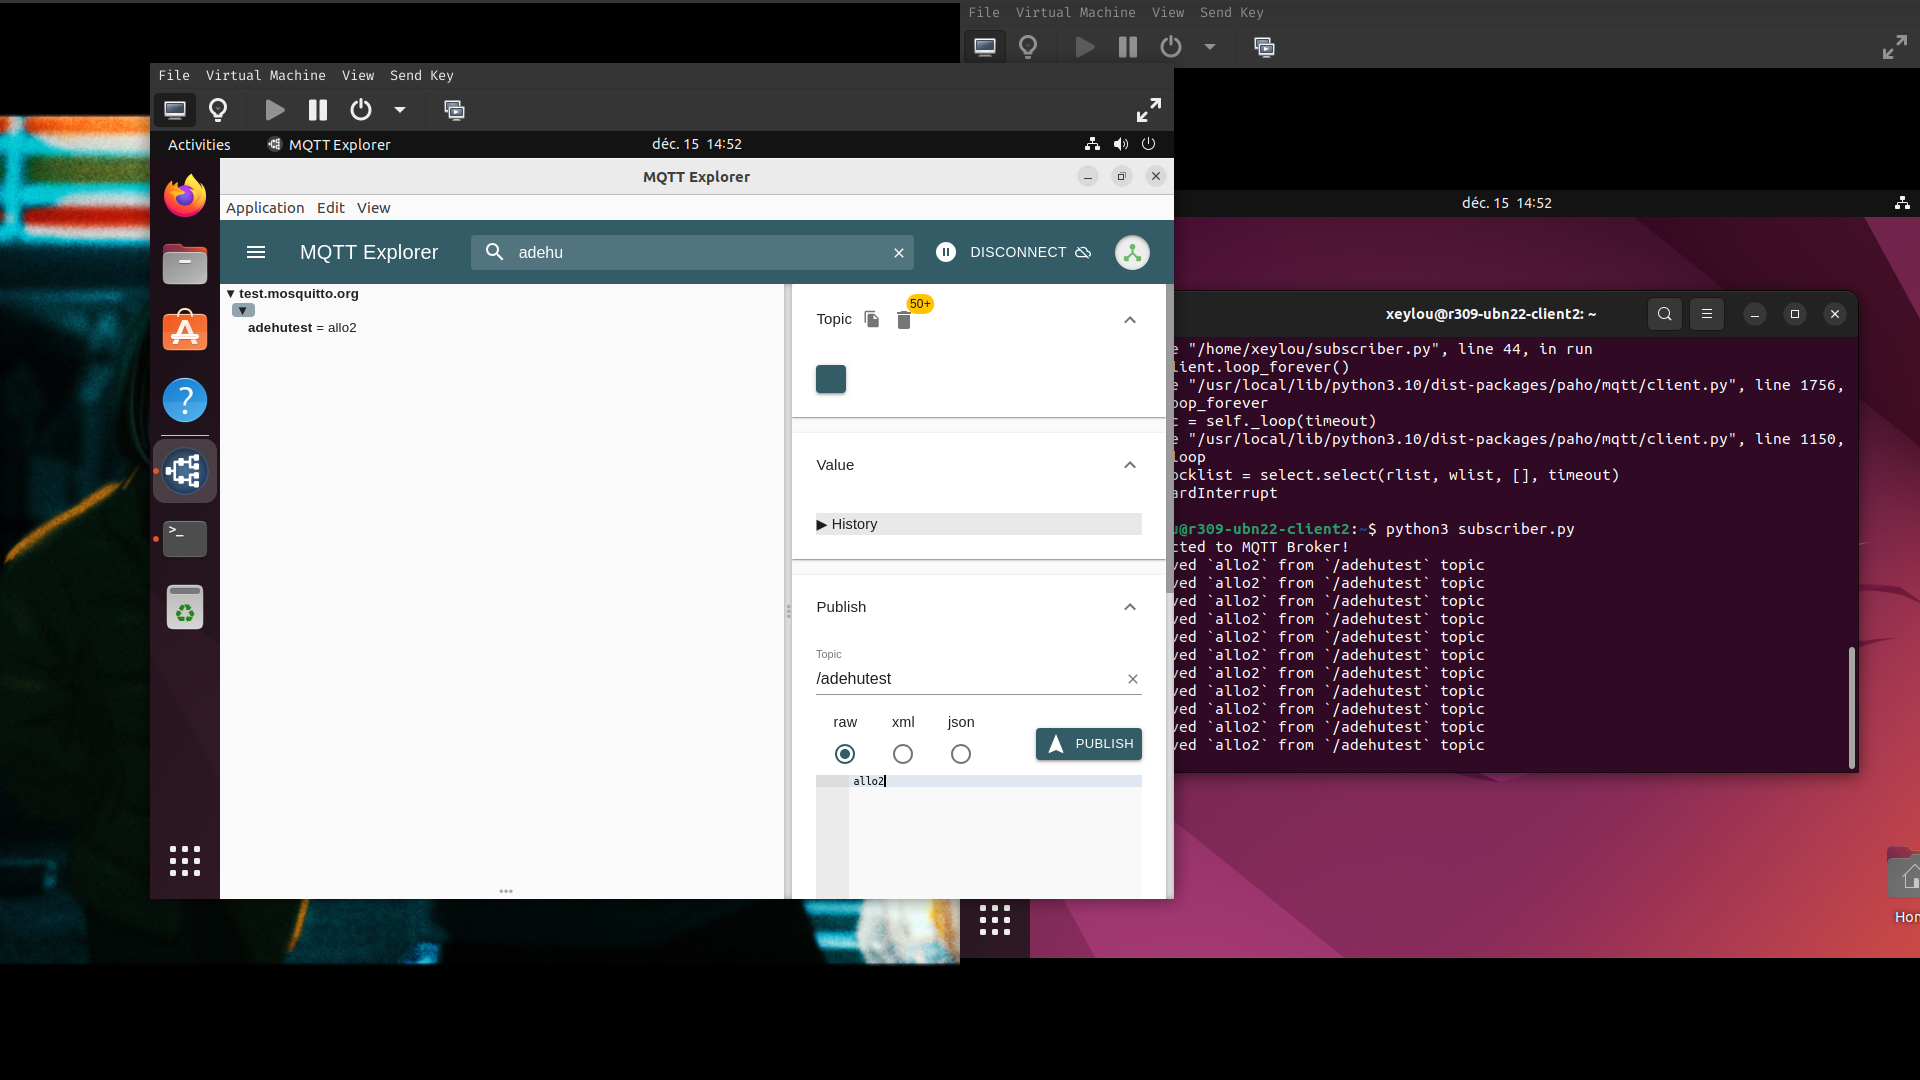
\includegraphics[width=\textwidth - \textwidth / 8]{ressources/r309/00.png}
      \caption{Utilisation de l'applicatif MQTT Explorer pour vérifier le fonctionnement d'un de mes scripts.}
      \label{fig:r309-00}
\end{figure}